\chapter{Evaluation}
\label{Evaluation}

\section{Objective of evaluation}

\section{Testing Environment}

\section{Methodology}

\section{Feasibility}

\section{}




Modifying handshake in DTLS is a bit tricky, as we want the data from TESLA to be protected and still be accepted by DTLS client and server. This is because DTLS client and server send a message flight "FINISHED", which contains MAC of previous message flights for integrity check. We need to make TESLA information be a part of this integrity check.

However, the signature size is too big to fit in the handshake messages, we therefore make amend to add TESLA initialization messages in first few packets of application data transfer. For this we modified the DTLS as shown in Fig \ref{hs}.


This was an experiment to check if sending buffer can send 21KB data, analyze wireshark traffic for fragmentation.

We see that application data can send buffer of maximum size limitation \footnote{In tinyDTLS, this maximum value is given by two constants DTLS\_MAX\_BUF(on read buffer size on server side) and MAX\_READ\_BUF(on read buffer size on client side)} same as in handshake data, that is, the UDP limit of 1500Bytes for ethernet and 65536($2^{16}$).\footnote{An UDP application may wish to avoid IP fragmentation, because when the size of the resulting datagram exceeds the link’s MTU, the IP datagram is split across multiple IP packets, which can lead to performance issues because if any fragment is lost, the entire datagram is lost.}

\begin{enumerate}
    \item The \textbf{first application data packet} contains \textbf{tesla synchronization request} with a nonce, a total of 32 Bytes flight.
    
    \item The \textbf{second application data packet} contains \textbf{tesla synchronization response} message with a nonce, a total of 181 Bytes flight.
    
\end{enumerate}  


 \begin{figure}[H]
    \centering
    \includegraphics[height=10cm,width=16cm]{figures/dtls-teslaHS(AppLayer).png}
    \caption{DTLS+TESLA Authentication mode using PSK}
    \label{hs}
    \end{figure}
    
\begin{enumerate}
    \item Setup (i): \\
    
               Machines: Ubuntu 16.04(Server) and Ubuntu 18.xx(Client) \\
               
               Maximum buffer sizes . :  $DTLS\_MAX\_BUF$ and $MAX\_READ\_BUF$ set to 30000(Bytes).\\
                
                File Size : 25KB, reading 150bytes per packet. This can be increased to read upto maximum buffer size.\\
                
               Results: Successful communication, data read from a file by client and sent it to server, with application data packets of size 30Kbytes. 
    \item Setup (ii): \\
    
               Machines: Ubuntu 16.04(Server) and MacOS(Client) \\
               
               Maximum buffer sizes . :  $DTLS\_MAX\_BUF$ and $MAX\_READ\_BUF$ set to 30000(Bytes).\\
                
                File Size : 25KB, reading 150bytes per packet. This can be increased to read upto maximum buffer size.\\
               
               Results: Unsuccessful communication, data read from a file by client and sent it to server, with handshake packets of size(any size).\\
               
              Reason for failure: The reason is that I think is because C executables are OS dependent, so when we compile and run it is not compatible. Also, MacOS does not allow any packets more than 1500bytes.
\end{enumerate}




\subsection{Experiment 2: Modified flights containing TESLA initialization}
We choose to work with changing the existing flights to accommodate TESLA packets. We add handshake maintaining state of the client and server after each message flight. Technically, there is no change in state of the original DTLS server or client, the handshake flights add TESLA data to the existing flights. 

We go ahead with the changing the existing handshake, this means that existing handshake message flights contains TESLA initialization messages.

\begin{enumerate}
    \item \textbf{ServerHello} contains \textbf{tesla synchronization request} with a nonce, a total of 32 Bytes addition to existing flight.
    
    \item \textbf{ClientKeyExchange} contains \textbf{tesla synchronization response} message with a nonce, a total of 181 Bytes addition to existing flight.
    
\end{enumerate}  


 \begin{figure}[H]
    \centering
    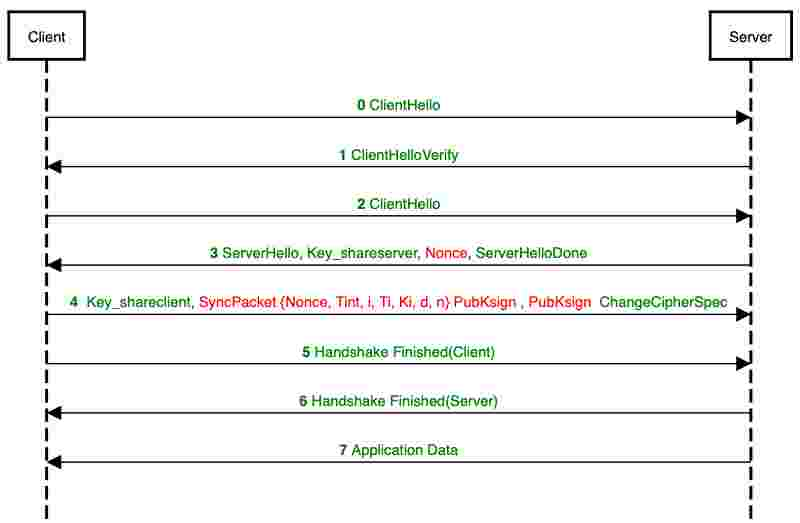
\includegraphics[height=10cm,width=16cm]{figures/hs.jpg}
    \caption{DTLS+TESLA Authentication mode using PSK}
    \label{hs}
    \end{figure}
    
    
    
\subsubsection{TESLA Parameters Selection}
Finally, the TESLA Initialization(89Bytes) consists of following values in the implementation :
\begin{enumerate}
    \item $Nonce$ : Generated using PRNG
    \item $T_{sender}$ : $dtls\_ticks()$ converted 4 bytes data. 
    \item $rate$ : Interval time is 1 packet/time interval. This is chosen after the rtt value is known.
    \item $i$ : Interval index starts at zero. 
    \item $T_{start}$ : Start time of sender corresponding to beginning of the session.
    The starting time of time interval i is thus $(T_{start} + i * T_{int})$.
    
    \item $n$ : Key chain length(taken as 1000). 
    
    \item $T_{int}$ : Interval duration .Practical values for $T_{int}$ vary from 100 milliseconds to 1 second.
    
    \item $d$ :Based on the RTT, the sender chooses a key disclosure delay $d$, where d denotes a number
   of time intervals, such that $d > ceil(RTT/T_{int})$.
   
   \item \textit{One-way key chain}: Each key of the one-way key chain is active in one time interval, for example, key $K_{i}$ is active in time interval $i$. The sender always uses the active key to compute the MAC of a packet it sends. The sender discloses the keys with a delay of $d$ time intervals, so it discloses key $K_{i-d}$ in
   time interval $i$.
   
    \item ECDSA signature and verification: ECDSA signature with 32byte key length and 64 byte signature is used. We implement existing ECDSA Signature in handshake for authenticating synchronization message. In TinyDTLS, we have a ECDSA signature implementation for P-256.
    
    
    
    
\end{enumerate}





\section{Cryptographic Primitives and Parameters(Updated) \cite{srtptesla}}
\begin{minipage}{18cm}
\begin{table}[H]
\caption{Cryptographic Primitives and Parameters(Updated) }
\label{cryptoTable}
\begin{tabular}{ |p{5cm}|p{5cm}|p{5cm}|}
\hline
\hline
\textbf{Crypto primitive} & \textbf{Algorithm Used} & \textbf{Used in / Used for}\\
 \hline
 \hline
\textit{Digital Signature} & $K2SN-MSS$(21.4 KB), ECDSA(64 Bytes) & $Tesla\_Sync$ \\ 
 \hline 
\textit{HMAC} & $HMAC-SHA-256$, keysize 32Bytes \href{https://tools.ietf.org/html/rfc2104}{RFC2104} & DTLSFinished
(Handshake Message), $TESLA-PRF$\\
\hline
\textit{TESLA-PRF} & $SHA-256$(blocksize 64bits and digest-size 32bits), keysize 32 Bytes & Key chain($K_{i}$), HMAC keys($K’_{i}$)\\
 \hline
 \textit{Hash} & $SHA-256$ & DTLS handshake integrity check\\
 
 \hline
 \textit{Encryption} & $AES-CCM-128$(keysize 16 and blocksize 16), output size 16Bytes & DTLS record layer\\
 \hline
 Maximum size of DTLS message & $DTLS\_MAX\_BUF$ & upto 44.1 KBytes (=65536 - 21400) Bytes excluding signature \\
 \hline
 Maximum Payload size & 16384($2^{14}$)Or 65536 ($2^{16}$)Bytes & DTLS-TESLA application data payload\\
\hline
 \textit{PRNG} & $Dtls\_fill\_random()$ that uses dev/urandom file in Linux (Refer : \href{http://cs.yale.edu/homes/aspnes/pinewiki/C(2f)Randomization.html}{CRandom}) & Nonce(used in TESLA) \\
 \hline
\end{tabular}\\

\end{table}
\end{minipage}    



